\documentclass[]{article}
\usepackage{lmodern}
\usepackage{amssymb,amsmath}
\usepackage{ifxetex,ifluatex}
\usepackage{fixltx2e} % provides \textsubscript
\ifnum 0\ifxetex 1\fi\ifluatex 1\fi=0 % if pdftex
  \usepackage[T1]{fontenc}
  \usepackage[utf8]{inputenc}
\else % if luatex or xelatex
  \ifxetex
    \usepackage{mathspec}
  \else
    \usepackage{fontspec}
  \fi
  \defaultfontfeatures{Ligatures=TeX,Scale=MatchLowercase}
\fi
% use upquote if available, for straight quotes in verbatim environments
\IfFileExists{upquote.sty}{\usepackage{upquote}}{}
% use microtype if available
\IfFileExists{microtype.sty}{%
\usepackage{microtype}
\UseMicrotypeSet[protrusion]{basicmath} % disable protrusion for tt fonts
}{}
\usepackage[margin=1in]{geometry}
\usepackage{hyperref}
\hypersetup{unicode=true,
            pdftitle={Score d'escarre en réanimation},
            pdfauthor={Philippe MICHEL},
            pdfborder={0 0 0},
            breaklinks=true}
\urlstyle{same}  % don't use monospace font for urls
\usepackage{longtable,booktabs}
\usepackage{graphicx,grffile}
\makeatletter
\def\maxwidth{\ifdim\Gin@nat@width>\linewidth\linewidth\else\Gin@nat@width\fi}
\def\maxheight{\ifdim\Gin@nat@height>\textheight\textheight\else\Gin@nat@height\fi}
\makeatother
% Scale images if necessary, so that they will not overflow the page
% margins by default, and it is still possible to overwrite the defaults
% using explicit options in \includegraphics[width, height, ...]{}
\setkeys{Gin}{width=\maxwidth,height=\maxheight,keepaspectratio}
\IfFileExists{parskip.sty}{%
\usepackage{parskip}
}{% else
\setlength{\parindent}{0pt}
\setlength{\parskip}{6pt plus 2pt minus 1pt}
}
\setlength{\emergencystretch}{3em}  % prevent overfull lines
\providecommand{\tightlist}{%
  \setlength{\itemsep}{0pt}\setlength{\parskip}{0pt}}
\setcounter{secnumdepth}{0}
% Redefines (sub)paragraphs to behave more like sections
\ifx\paragraph\undefined\else
\let\oldparagraph\paragraph
\renewcommand{\paragraph}[1]{\oldparagraph{#1}\mbox{}}
\fi
\ifx\subparagraph\undefined\else
\let\oldsubparagraph\subparagraph
\renewcommand{\subparagraph}[1]{\oldsubparagraph{#1}\mbox{}}
\fi

%%% Use protect on footnotes to avoid problems with footnotes in titles
\let\rmarkdownfootnote\footnote%
\def\footnote{\protect\rmarkdownfootnote}

%%% Change title format to be more compact
\usepackage{titling}

% Create subtitle command for use in maketitle
\newcommand{\subtitle}[1]{
  \posttitle{
    \begin{center}\large#1\end{center}
    }
}

\setlength{\droptitle}{-2em}

  \title{Score d'escarre en réanimation}
    \pretitle{\vspace{\droptitle}\centering\huge}
  \posttitle{\par}
    \author{Philippe MICHEL}
    \preauthor{\centering\large\emph}
  \postauthor{\par}
    \date{}
    \predate{}\postdate{}
  

\begin{document}
\maketitle

{
\setcounter{tocdepth}{2}
\tableofcontents
}
\hypertarget{protocole}{%
\section{Protocole}\label{protocole}}

Pour établir un score de gravté il faut disposer de variables toutes
factorielles, idéalement binaires, sinon ordonnées avec peu de valeurs
possibles. Ces variables seront toutes celles parraissant significatives
avec un seuil assez élevé (p \textless{}0,2 par ex.).

Ensuite, sur un premeir groupe de patients pris dns l'échantillon total
(autour de 1/3) on recherche par régression logistique une formule
simple. Ensite on teste cette frmule sur le reste de l'échantillon voire
un pseudo échantillon beaucoup plus grand obtenu par bootstrap ou autre.

\hypertarget{importation-mise-en-forme-des-variables}{%
\section{Importation \& mise en forme des
variables}\label{importation-mise-en-forme-des-variables}}

On ne garde que les patients n'ayant pas d'escarre à l'admission.

\hypertarget{facteurs-de-risque-connus}{%
\section{Facteurs de risque connus}\label{facteurs-de-risque-connus}}

Pour mémoire les facteurs de risque d'escarre mis en évidence dans
Pressure sont (en plus de l'IGS II):

\begin{itemize}
\tightlist
\item
  Sexe
\item
  Alité 7jours avant l'admission
\item
  Poids
\item
  Albumine
\item
  CRP
\item
  Ventilation
\item
  Corticoïdes
\item
  maladie neurologique
\item
  Type de nutrition
\end{itemize}

Pour mémoire, en régression, les facteurs retrouvés sont :

\begin{itemize}
\tightlist
\item
  Poids \textgreater{} 90 Kg
\item
  Corticoïdes
\item
  Maladie neurologique
\end{itemize}

\hypertarget{recherche-de-seuils}{%
\section{Recherche de seuils}\label{recherche-de-seuils}}

Pour les variables numériques (poids, albumine, CRP), on recherche un
seuil * significatif * par les courbes de ROC.

Malheureusement ces trois variables ont des courbes ROC très plates sans
seuil bien défini. Néanmoins des seuils un peu moins mauvais ont pu être
trouvés :

\begin{itemize}
\tightlist
\item
  Poids : 90 Kg
\item
  Albumine: 23
\item
  CRP : 90
\end{itemize}

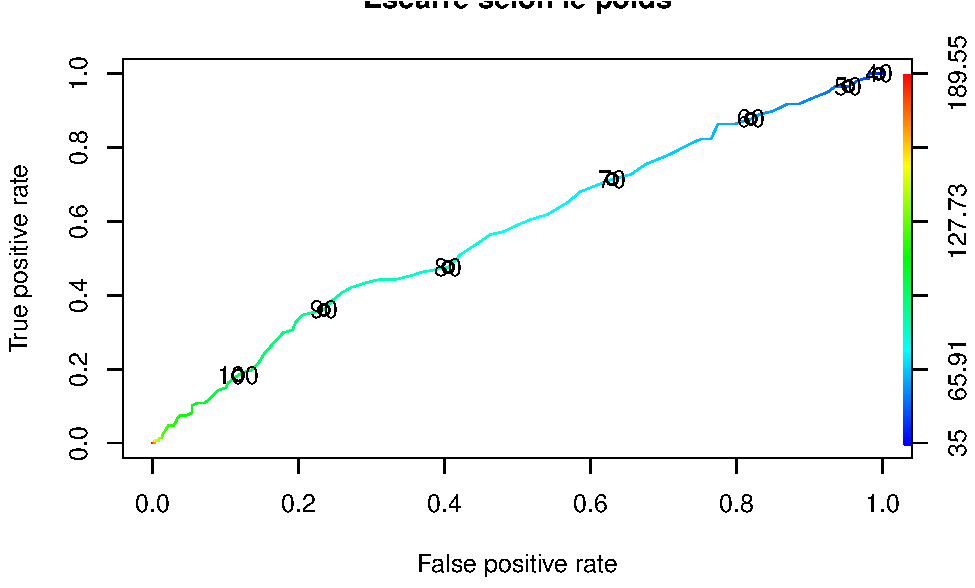
\includegraphics{book_escarre_files/figure-latex/roc-1.pdf}
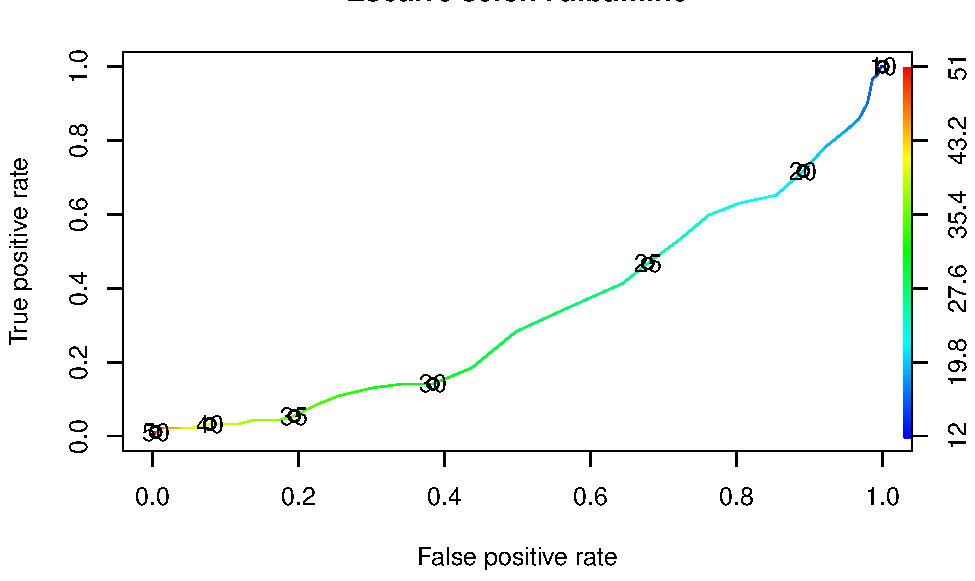
\includegraphics{book_escarre_files/figure-latex/roc-2.pdf}
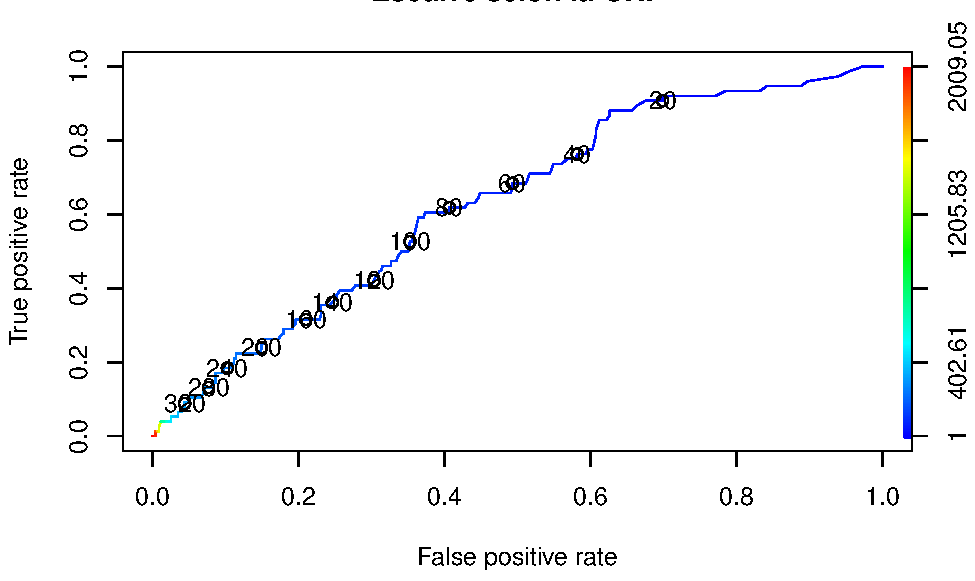
\includegraphics{book_escarre_files/figure-latex/roc-3.pdf}
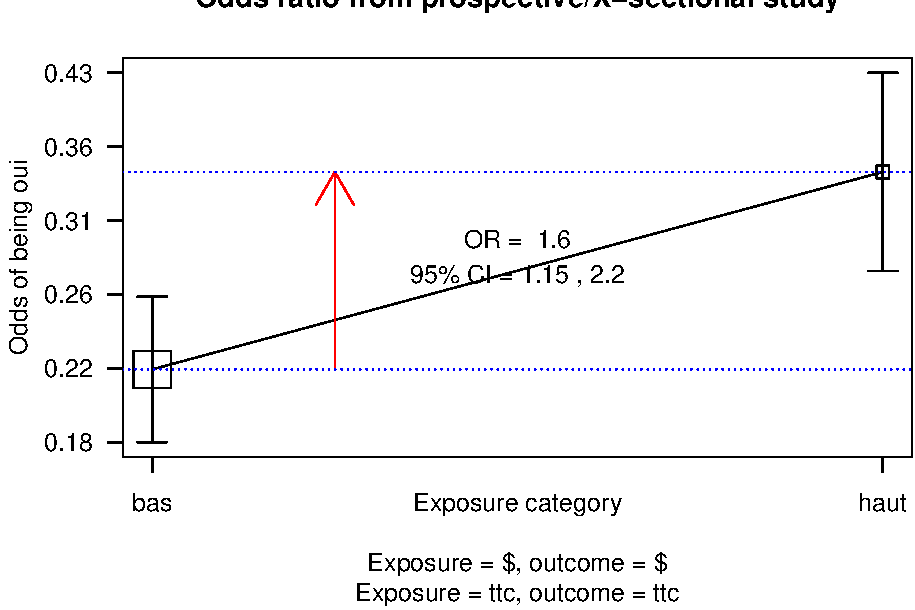
\includegraphics{book_escarre_files/figure-latex/roc-4.pdf}

\begin{verbatim}
## 
##             ttc$poids
## ttc$escarrej  bas haut Total
##        non    729  224   953
##        oui     94   53   147
##        Total  823  277  1100
## 
## OR =  1.83 
## Exact 95% CI =  1.24, 2.69  
## Chi-squared = 10.65, 1 d.f., P value = 0.001
## Fisher's exact test (2-sided) P value = 0.002
\end{verbatim}

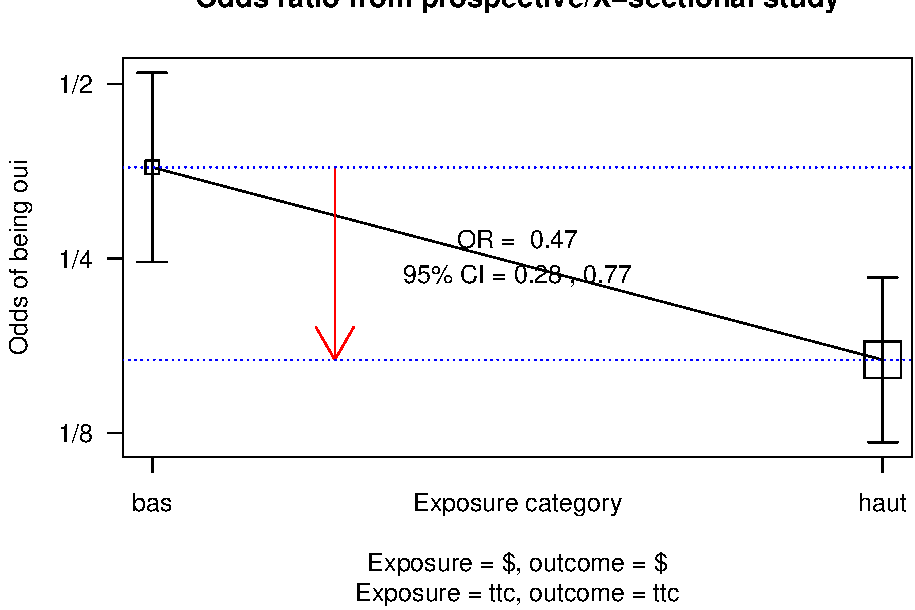
\includegraphics{book_escarre_files/figure-latex/roc-5.pdf}

\begin{verbatim}
## 
##             ttc$albumine
## ttc$escarrej bas haut Total
##        non   103  329   432
##        oui    37   55    92
##        Total 140  384   524
## 
## OR =  0.47 
## Exact 95% CI =  0.28, 0.77  
## Chi-squared = 10.39, 1 d.f., P value = 0.001
## Fisher's exact test (2-sided) P value = 0.002
\end{verbatim}

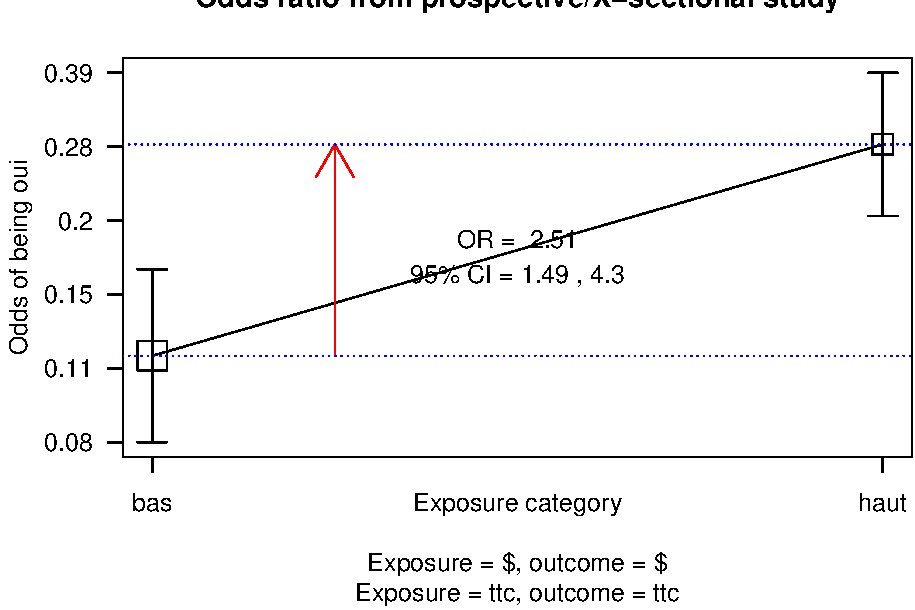
\includegraphics{book_escarre_files/figure-latex/roc-6.pdf}

\begin{verbatim}
## 
##             ttc$crp
## ttc$escarrej bas haut Total
##        non   266  162   428
##        oui    30   46    76
##        Total 296  208   504
## 
## OR =  2.52 
## Exact 95% CI =  1.49, 4.3  
## Chi-squared = 13.69, 1 d.f., P value = 0
## Fisher's exact test (2-sided) P value = 0
\end{verbatim}

On dispose ainsi de variables factorielles simples, binaires pour tous
les facteurs à étudier

\hypertarget{regression-logistique-preparatoire}{%
\section{Régression logistique
(préparatoire)}\label{regression-logistique-preparatoire}}

Pour ces travaux préparatoires j'utilise tout l'échantillon. Le
protocole complet ne sear utilisé que lorsqu'un score semblera être
meilleur. On lance la régression sur les variables retenues.

\hypertarget{sans-ponderation}{%
\subsection{Sans pondération}\label{sans-ponderation}}

\begin{verbatim}
##  
##                         OR lower95ci upper95ci     Pr(>|Z|)
## alité.avantoui   1.6339184 0.7191463  3.712304 0.2409632302
## sexeH            0.9938392 0.4525917  2.182356 0.9877142044
## poidshaut        1.9957780 0.9013998  4.418827 0.0883825700
## albuminehaut     0.5861868 0.2605712  1.318699 0.1966372230
## crphaut          2.9949207 1.3831575  6.484836 0.0053876879
## ventilationoui   1.6331787 0.5556340  4.800414 0.3725487138
## corticoïdesoui   2.8577732 1.3239041  6.168776 0.0074802707
## déficit.neurooui 4.3943241 1.9180049 10.067797 0.0004657575
## nutritionper.os  0.4216763 0.1468089  1.211172 0.1086988832
\end{verbatim}

Si on ne retint que les variables significatives on garde : alité avant,
poids, corticoïdes, déficit neurologique. En donnant le même poids à
toute les variables on obtient un score simple à quatre items noté de 0
à 4.

\begin{longtable}[]{@{}rrrrr@{}}
\toprule
score & n & risque & binf & bsup\tabularnewline
\midrule
\endhead
0 & 390 & 4.6 & 2.8 & 7.2\tabularnewline
1 & 373 & 12.9 & 9.6 & 16.7\tabularnewline
2 & 181 & 26.0 & 19.7 & 33.0\tabularnewline
3 & 43 & 48.8 & 33.3 & 64.5\tabularnewline
4 & 2 & 100.0 & 15.8 & 100.0\tabularnewline
\bottomrule
\end{longtable}

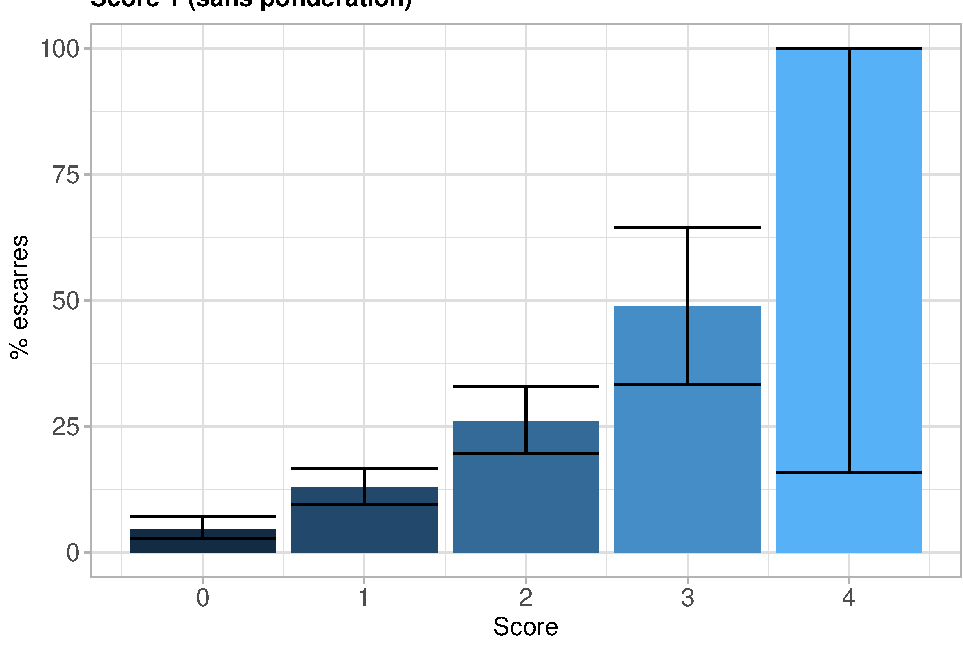
\includegraphics{book_escarre_files/figure-latex/unnamed-chunk-2-1.pdf}

\hypertarget{avec-ponderation}{%
\subsection{Avec pondération}\label{avec-ponderation}}

On applique une pondération basée sur les OD en gardant les mêmes items.
On obtient donc alite avant x 2 + poids x 2 + corticïdes x 2 + deficit
neuro x 3

Le plus grand nombre de niveaux rend la lecture moins nette, il faudra
prévoir des regroupements de niveau.

\begin{longtable}[]{@{}lrrrr@{}}
\toprule
score & n & risque & binf & bsup\tabularnewline
\midrule
\endhead
0 & 390 & 4.6 & 2.8 & 7.2\tabularnewline
2 & 277 & 10.1 & 6.8 & 14.3\tabularnewline
3 & 96 & 20.8 & 13.2 & 30.3\tabularnewline
4 & 89 & 23.6 & 15.2 & 33.8\tabularnewline
5 & 92 & 28.3 & 19.4 & 38.6\tabularnewline
6 & 8 & 50.0 & 15.7 & 84.3\tabularnewline
7 & 35 & 48.6 & 31.4 & 66.0\tabularnewline
9 & 2 & 100.0 & 15.8 & 100.0\tabularnewline
\bottomrule
\end{longtable}

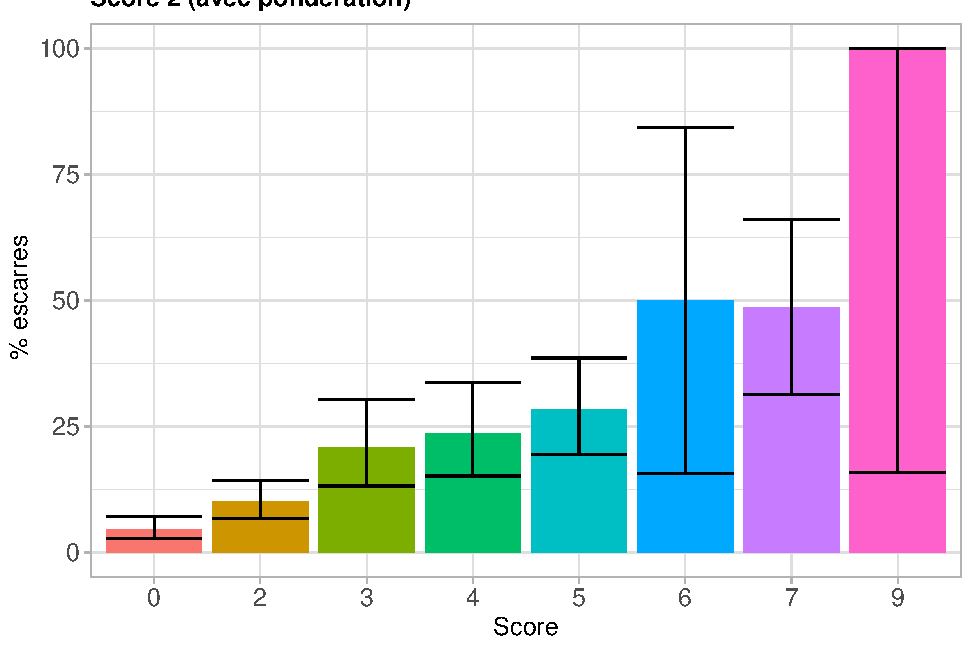
\includegraphics{book_escarre_files/figure-latex/sc2-1.pdf}

\hypertarget{scores-habituels}{%
\subsection{Scores ``habituels''}\label{scores-habituels}}

Pour avoir un point de comparaison, voici la prédiction obtenue dans
PRESSURE par l'échelle habituelle du service.

\begin{tabular}{lrrrr}
\toprule
score & n & risque & binf & bsup\\
\midrule
Pas de risque & 99 & 0.0 & 0.0 & 3.7\\
Risque faible & 298 & 3.7 & 1.9 & 6.5\\
Risque moyen & 378 & 9.3 & 6.5 & 12.6\\
Risque élevé & 387 & 26.9 & 22.5 & 31.6\\
\bottomrule
\end{tabular}

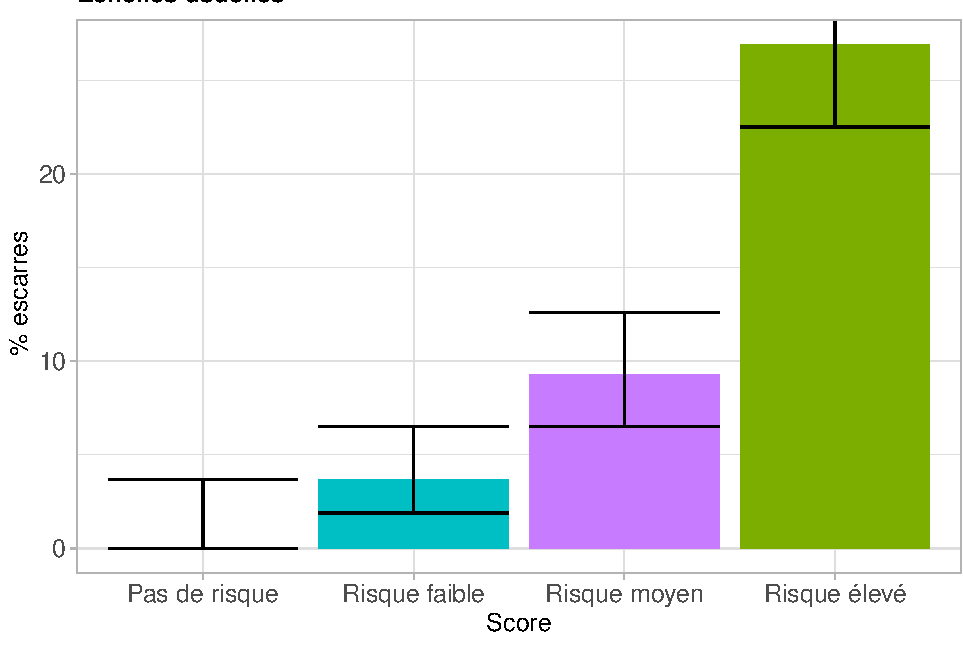
\includegraphics{book_escarre_files/figure-latex/schab-1.pdf} \#\#
Validation des seuils

Pour chacun des deux scores étudiés on cherche le moins mauvais seuil.

\hypertarget{score-non-modere}{%
\subsection{Score non modéré}\label{score-non-modere}}

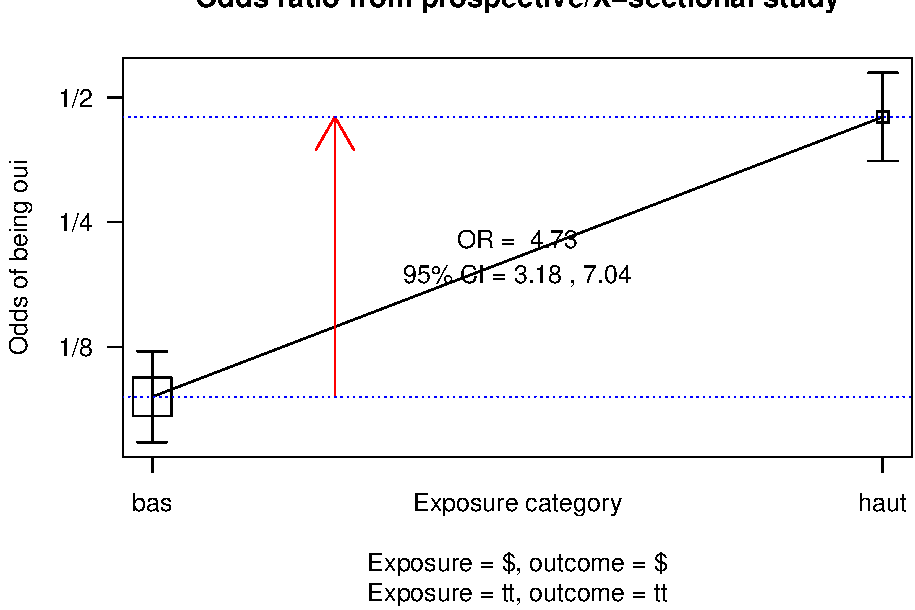
\includegraphics{book_escarre_files/figure-latex/seuil1-1.pdf}

\begin{verbatim}
## 
##            tt$seuil11
## tt$escarrej bas haut Total
##       non   697  156   853
##       oui    66   70   136
##       Total 763  226   989
## 
## OR =  4.74 
## Exact 95% CI =  3.18, 7.04  
## Chi-squared = 73.26, 1 d.f., P value = 0
## Fisher's exact test (2-sided) P value = 0
\end{verbatim}

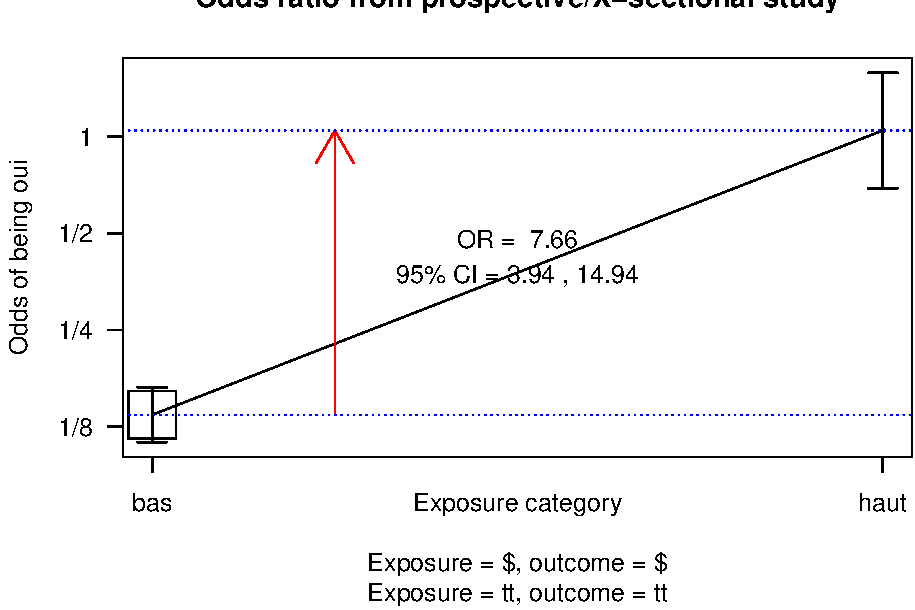
\includegraphics{book_escarre_files/figure-latex/seuil1-2.pdf}

\begin{verbatim}
## 
##            tt$seuil12
## tt$escarrej bas haut Total
##       non   831   22   853
##       oui   113   23   136
##       Total 944   45   989
## 
## OR =  7.69 
## Exact 95% CI =  3.94, 14.94  
## Chi-squared = 55.48, 1 d.f., P value = 0
## Fisher's exact test (2-sided) P value = 0
\end{verbatim}

Le seuil \textless{}=3 semble plus discriminant avec 11 \%
{[}9,9;14,2{]} d'escarre dans le groupe à faible risque vs 48,9 \%
{[}33,7;64,2{]} dans le groupe à haut risque.

\hypertarget{score-pondere}{%
\subsection{Score pondéré}\label{score-pondere}}

En essayant tous les seuils posiibles le meilleur OD est trouvé pour
\textgreater{}=6 avec 12,0 \% {[}10,0;14,2{]} d'escarre dans le groupe à
bas risque vs 51,1 \% {[}35,8;66,2{]} pour le groupe à haut risque.
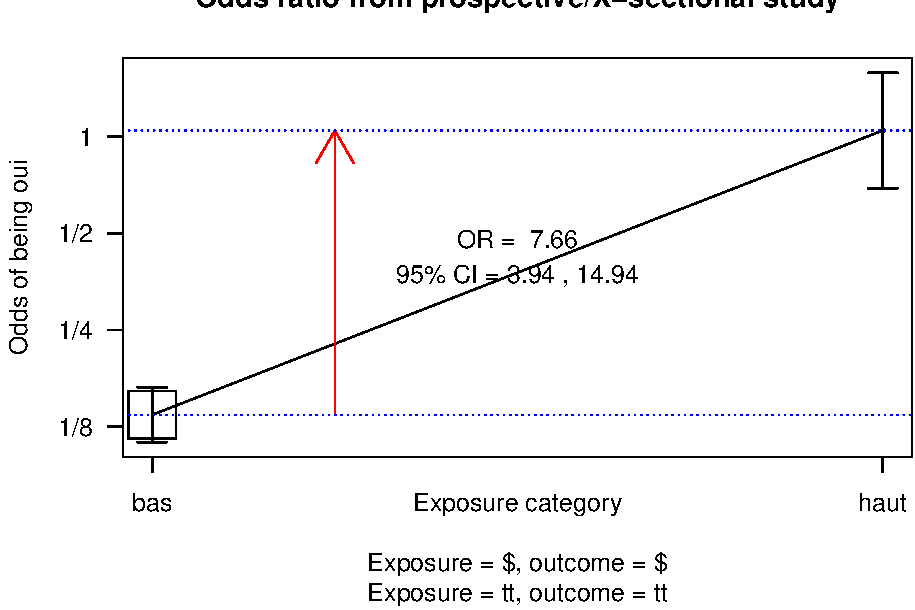
\includegraphics{book_escarre_files/figure-latex/seuil2-1.pdf}

\begin{verbatim}
## 
##            tt$seuil2
## tt$escarrej bas haut Total
##       non   831   22   853
##       oui   113   23   136
##       Total 944   45   989
## 
## OR =  7.69 
## Exact 95% CI =  3.94, 14.94  
## Chi-squared = 55.48, 1 d.f., P value = 0
## Fisher's exact test (2-sided) P value = 0
\end{verbatim}

\hypertarget{conclusion}{%
\section{Conclusion}\label{conclusion}}

Les scores proposés isolent plus de patients avec un risque faible que
les échelles habituelles. Donc un intérêt économique (moins de patients
chez qui utiliser des méthodes de préventrions complexes \& chères).


\end{document}
